\documentclass[compress]{beamer}
\usepackage{ifthen}

\title{Status of Muon Chambers in CommonAlignment}
\author{Jim Pivarski}
\institute{Texas A\&M University}
\date{16 February, 2007}

\setbeamertemplate{navigation symbols}{}
\setbeamertemplate{headline}{\includegraphics[height=1 cm]{../cmslogo} \hspace{0.1 cm} \includegraphics[height=1 cm]{../tamulogo} \hfill
\begin{minipage}{9 cm}
\vspace{-0.75 cm} \small
\begin{center}
\ifthenelse{\equal{\insertpagenumber}{1}}{}{\insertsection}
\end{center}
\end{minipage} \hfill
\begin{minipage}{1 cm}
\vspace{-0.75 cm} \small
\begin{center}
\ifthenelse{\equal{\insertpagenumber}{1}}{}{\insertpagenumber/\pageref{numpages}}
\end{center}
\end{minipage}}

%% \xdefinecolor{verylightgray}{rgb}{0.95,0.95,0.95}
%% \beamertemplateshadingbackground{verylightgray}{white}

\begin{document}
\frame{\titlepage}
\section*{Muon Chambers in CommonAlignment --- Jim Pivarski}



\begin{frame}
  \frametitle{Muon Alignment System in CommonAlignment}

  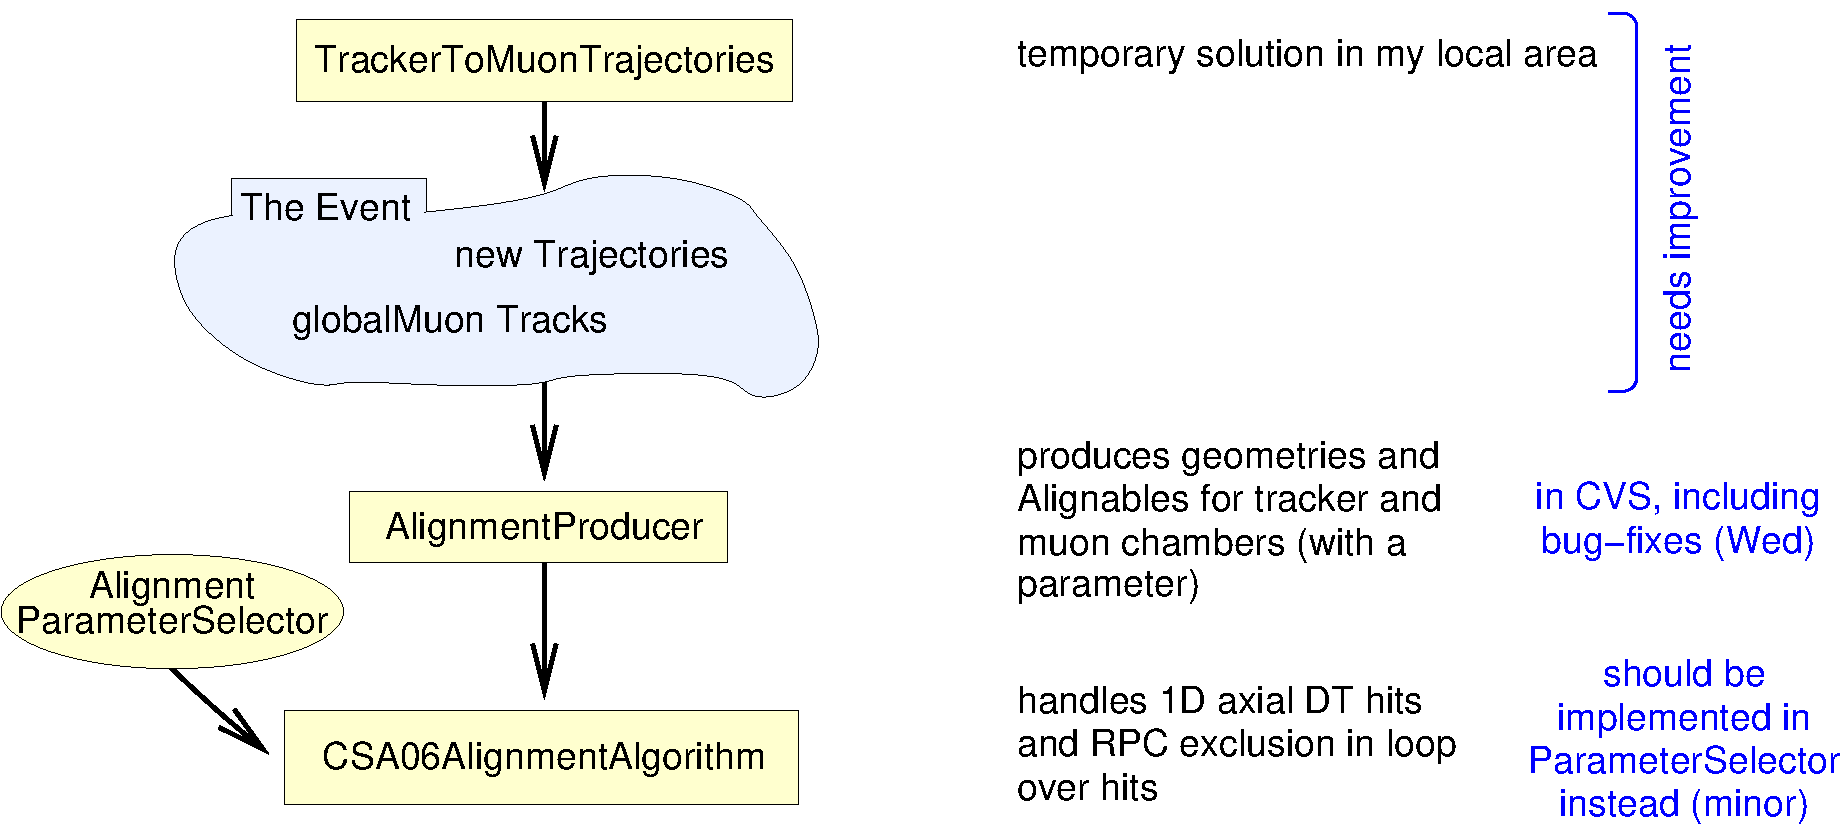
\includegraphics[width=\linewidth]{system_with_muons}

  \begin{itemize}
    \item System works in my local area
    \item We want to put a working and acceptable system into CVS \mbox{as soon as possible}
  \end{itemize}

\end{frame}


\begin{frame}
  \frametitle{Temporary Solution for Trajectory-Making}

  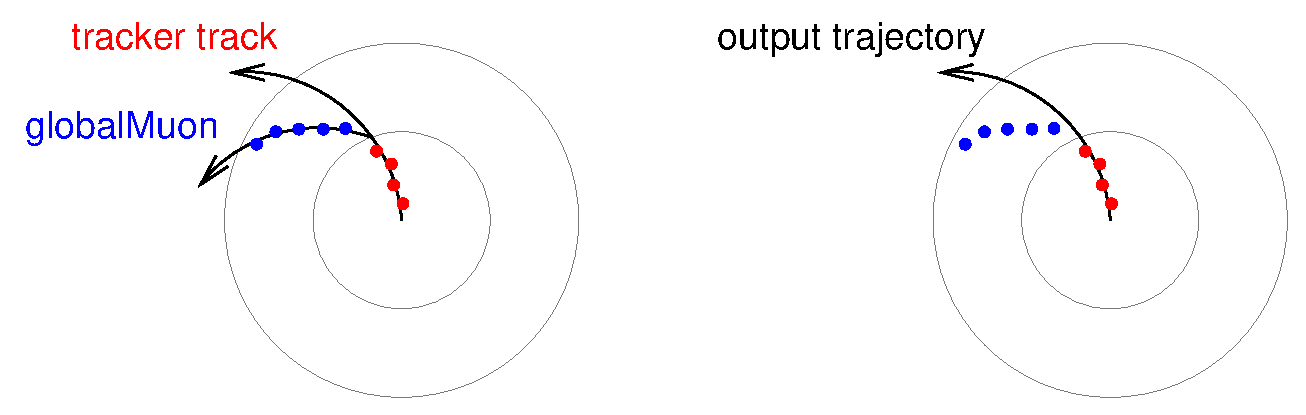
\includegraphics[width=\linewidth]{making_trajectories}

  \begin{itemize}\setlength{\itemsep}{0.25 cm}
    \item Unbiased by muon hits $\to$ fewer HIP iterations
    \item This is the trackerfit-only extreme, StandAloneMuon-only extreme is also easy to implement
    \item Optimal fit is some $(1-\alpha)$ trackerfit $+$ $\alpha$ muonfit
  \end{itemize}
How should we implement that?
\end{frame}

\begin{frame}
  \frametitle{Implementing $(1-\alpha)$ trackerfit $+$ $\alpha$ muonfit}

\begin{itemize}
\item With GlobalMuonProducer?
\end{itemize}

\vfill
\fbox{\begin{minipage}{\linewidth}
\small \tt
module globalMuonsForAlignment = GlobalMuonProducer \\
\{ \\
\mbox{\hspace{0.5 cm}}InputTag MuonCollectionLabel = standAloneMuons \\
\mbox{\hspace{0.5 cm}}InputTag TrackerCollectionLabel = ctfWithMaterialTracks \\
\mbox{\hspace{0.5 cm}}PSet TrackLoaderParameters = \\
\mbox{\hspace{0.5 cm}}\{ \\
\mbox{\hspace{0.5 cm}}\mbox{\hspace{0.5 cm}}untracked bool PutTrajectoryIntoEvent = \textcolor{blue}{true} \\
\mbox{\hspace{0.5 cm}}\} \\
\mbox{\hspace{0.5 cm}}\textcolor{blue}{double MuonWeightInFit = 0.5}
\end{minipage}}

\vfill
\begin{itemize}
\item With a new producer in RecoMuon?
\end{itemize}

\vfill
I should talk with Riccardo again\ldots
\end{frame}

\begin{frame}
\frametitle{Muon Geometry in AlignmentProducer}
\begin{itemize}\setlength{\itemsep}{0.5 cm}
  \item AlignmentProducer has two new parameters: \begin{center} doTracker (bool) \mbox{\hspace{0.3 cm}} and \mbox{\hspace{0.3 cm}} doMuon (bool) \end{center}
  \item With doMuon, it produces DTGeometry and CSCGeometry
  \item Applies muon misalignment scenarios, saves to database, etc.\ (completely parallel to tracker)
  \item Passes AlignableMuon to the concrete algorithms \\ (HIP, MillePede, Kalman)
\end{itemize}

\vfill
All AlignmentProducer updates have been committed to CVS

\vfill
(including two bug fixes last Wednesday)
\end{frame}

\begin{frame}
\frametitle{Changes to CSA06AlignmentAlgorithm}
\textcolor{red}{These changes are only in my local area, not CVS.}

\vfill
\begin{itemize}\setlength{\itemsep}{0.5 cm}
  \item Axial DT hits have $z =$ center of chamber and ${\sigma_z}^2 = 0$
    \begin{itemize}\setlength{\itemsep}{0.25 cm}
      \item Okay for rphi alignment, bad for $z$ alignment
      \item I set $1/{\sigma_z}^2 = 0$ for these hits in sum over residuals
      \item Instead, we must tell AlignmentParameterSelector/Builder \mbox{to apply}
      these hits to rphi alignment, but not $z$
    \end{itemize}

  \item Tracks from some sources include RPC hits
    \begin{itemize}\setlength{\itemsep}{0.25 cm}
      \item I have excluded them from the loop over hits
      \item Also should be solved with AlignmentParameterSelector/Builder
      \item Perhaps RPC hits shouldn't be in offline tracks?
    \end{itemize}
\end{itemize}
\end{frame}


\begin{frame}
  \frametitle{Alignment Test with 6000 Muons}

  Alignment corrections, starting from\ldots

  \begin{tabular}{p{0.45\linewidth} p{0.45\linewidth}}
    \begin{minipage}{\linewidth}
      \begin{center}
	an ideal alignment
      \end{center}
    \end{minipage} &
    \begin{minipage}{\linewidth}
      \begin{center}
	\only<1>{all chambers $\Delta x = +1$ cm}
	\only<2>{all $\Delta \phi_z = +10$ mrad}
      \end{center}
    \end{minipage} \\
    \begin{minipage}{\linewidth}
      \begin{center}
	\only<1>{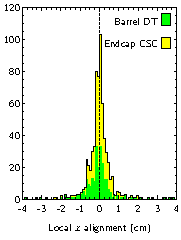
\includegraphics[width=\linewidth]{init_alignments_x}}
	\only<2>{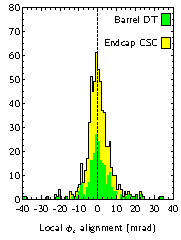
\includegraphics[width=\linewidth]{init_alignments_phiz}}
      \end{center}
    \end{minipage} &
    \begin{minipage}{\linewidth}
      \begin{center}
	\only<1>{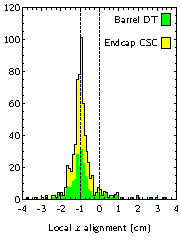
\includegraphics[width=\linewidth]{x_alignments_x}}
	\only<2>{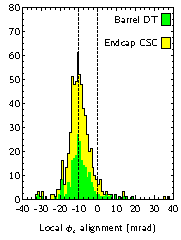
\includegraphics[width=\linewidth]{phiz_alignments_phiz}}
      \end{center}
    \end{minipage} 
  \end{tabular}
\end{frame}

\begin{frame}
\frametitle{Next Steps in Software Development}
I should\ldots

\vfill
\begin{itemize}\setlength{\itemsep}{0.5 cm}
  \item Ask Riccardo what is the best way to implement
  \mbox{globalMuons with} partially-weighted muon chambers

  \item Look at AlignmentParameterSelector/Builder and try to implement
  1D DT hits in the same way as 1D SiStrip hits (asking Gero for help,
  if needed)

  \item Exclude RPC hits in AlignmentParameterSelector/Builder

  \item Submit a working and acceptable system to CVS

  \item Write a Twiki page
\end{itemize}
\end{frame}

\begin{frame}
\frametitle{Next-After-Next Steps}
\begin{itemize}\setlength{\itemsep}{0.5 cm}
  \item Coordinate with Frederic and Reco groups to add AssociationMap$<$Tracks,Trajectories$>$

  \item CSA06 $\to$ HIPAlignmentAlgorithm

  \item Add a suite of diagnostic plots (to HIPAlignmentAlgorithm? or the whole framework? as an optional extension?)

  \item Help define the muon alignment data stream

    (Currently contains only StandAloneMuons)
\end{itemize}
\label{numpages}
\end{frame}

\end{document}
